\section*{Informations générales}
 
\begin{table}[h]
\centering
	\begin{tabularx}{16.8cm}{|X|X|}
	\hline
	Numéro de l'opportunité & Type d'opportunité \\
	\hline
	003 & Bonne passation \\
	\hline
	\end{tabularx}
\end{table}

\begin{table}[h]
\centering
	\begin{tabularx}{16.8cm}{|X|X|X|}
	\hline
	Date & Visa du \RQ & Visa du \CP \\
	\hline
	 07/12/15 & pgpic & pgpic \\
	\hline
	\end{tabularx}
\end{table}

\begin{table}[h]
\centering
	\begin{tabularx}{16.8cm}{|X|X|X|X|}
	\hline
	Pilote & Activité WBS & Compte WBS & Phase d'apparition \\
	\hline
	 \Pierre & Suivre les Risques et Opportunités & 1.2.3.2 & A partir de la fin du premier semestre.\\
	\hline
	\end{tabularx}
\end{table}

\section*{Description du risque}

\subsection*{Résumé}
	Grâce à une bonne passation, le temps de prise en main du projet par la nouvelle équipe pourrait être grandement réduit.
	
\subsection*{Analyse des causes}
	voir figure.

\subsection*{Criticité}

\begin{table}[h]
\centering
	\begin{tabularx}{12.8cm}{|>{
	%\columncolor{gray!40}
	}X|X|}
	\hline
	Bénéfice & 3\\
	\hline
	Probabilité & 3\\
	\hline
	Criticité & Important\\
	\hline
	\end{tabularx}
\end{table}
\newpage

\section*{Actions}
\subsection*{Actions proactives}

%\begin{table}[H]
\centering
	\begin{longtable}{|p{7cm}|p{7cm}|}
	\hline
	Cause & Actions proactives \\
	\hline
	 Rédaction de documents de passation & \begin{itemize}
	 	\item Attribuer de cette tâche
	 	\item Inclure de cette tâche dans le planning
	 	\item Commencer cette tâche à temps
	 \end{itemize} \\
	\hline
	Arrivée de la nouvelle équipe avant départ de l'ancienne & \begin{itemize}
		\item Demander à la nouvelle équipe d'arriver au plus tôt
	\end{itemize} \\
	\hline
	Communication préalable avec la nouvelle équipe & \begin{itemize}
		\item Organiser des rendez-vous téléphoniques
		\item Prévenir la nouvelle équipe de ces rendez-vous
	\end{itemize} \\
	\hline
	Passation prévue et organisée & \begin{itemize}
		\item Réfléchir au processus de passation
		\item Inclure la préparation de la passation dans le planning
		\item Nommer un responsable de la passation
	\end{itemize} \\
	\hline
	Mise en place d'outils de communication performants & \begin{itemize}
		\item Rechercher les outils les plus adaptés
		\item Tester différents outils
	\end{itemize} \\
	\hline
	Bon investissement de la nouvelle équipe & 
	 \\
	\hline
	Bonne planification & \begin{itemize}
		\item Former le \CP à la planification
		\item Bien prévoir les temps nécessaires à chaque tâche
	\end{itemize} \\
	\hline
	Bon investissement de l'ancienne équipe & 
	 \\
	\hline

	\end{longtable}
%\end{table}

\subsection*{Plan de contournement}

\begin{enumerate}
	\item Bloquer le site
	\item Demander un serveur temporaire
	\item Faire les démarches nécessaires pour les réparations
	\item Relancer le site
\end{enumerate}

\section*{Décision de clôture}
Par le \CP{} et le pilote du risque.
\begin{table}[h]
\centering
	\begin{tabularx}{16.8cm}{|X|X|}
	\hline
	Date de clôture & Raison de la clôture \\
	\hline
	  & \\
	\hline
	\end{tabularx}
\end{table}

\section*{Historique des modifications}
\begin{table}[h]
\centering
	\begin{tabularx}{16.8cm}{|X|X|}
	\hline
	Date & Modification \\%\rowcolor{gray!40} 
	\hline
	  & \\
	\hline
	\end{tabularx}
\end{table}
\newpage


\begin{figure}
	\centering
	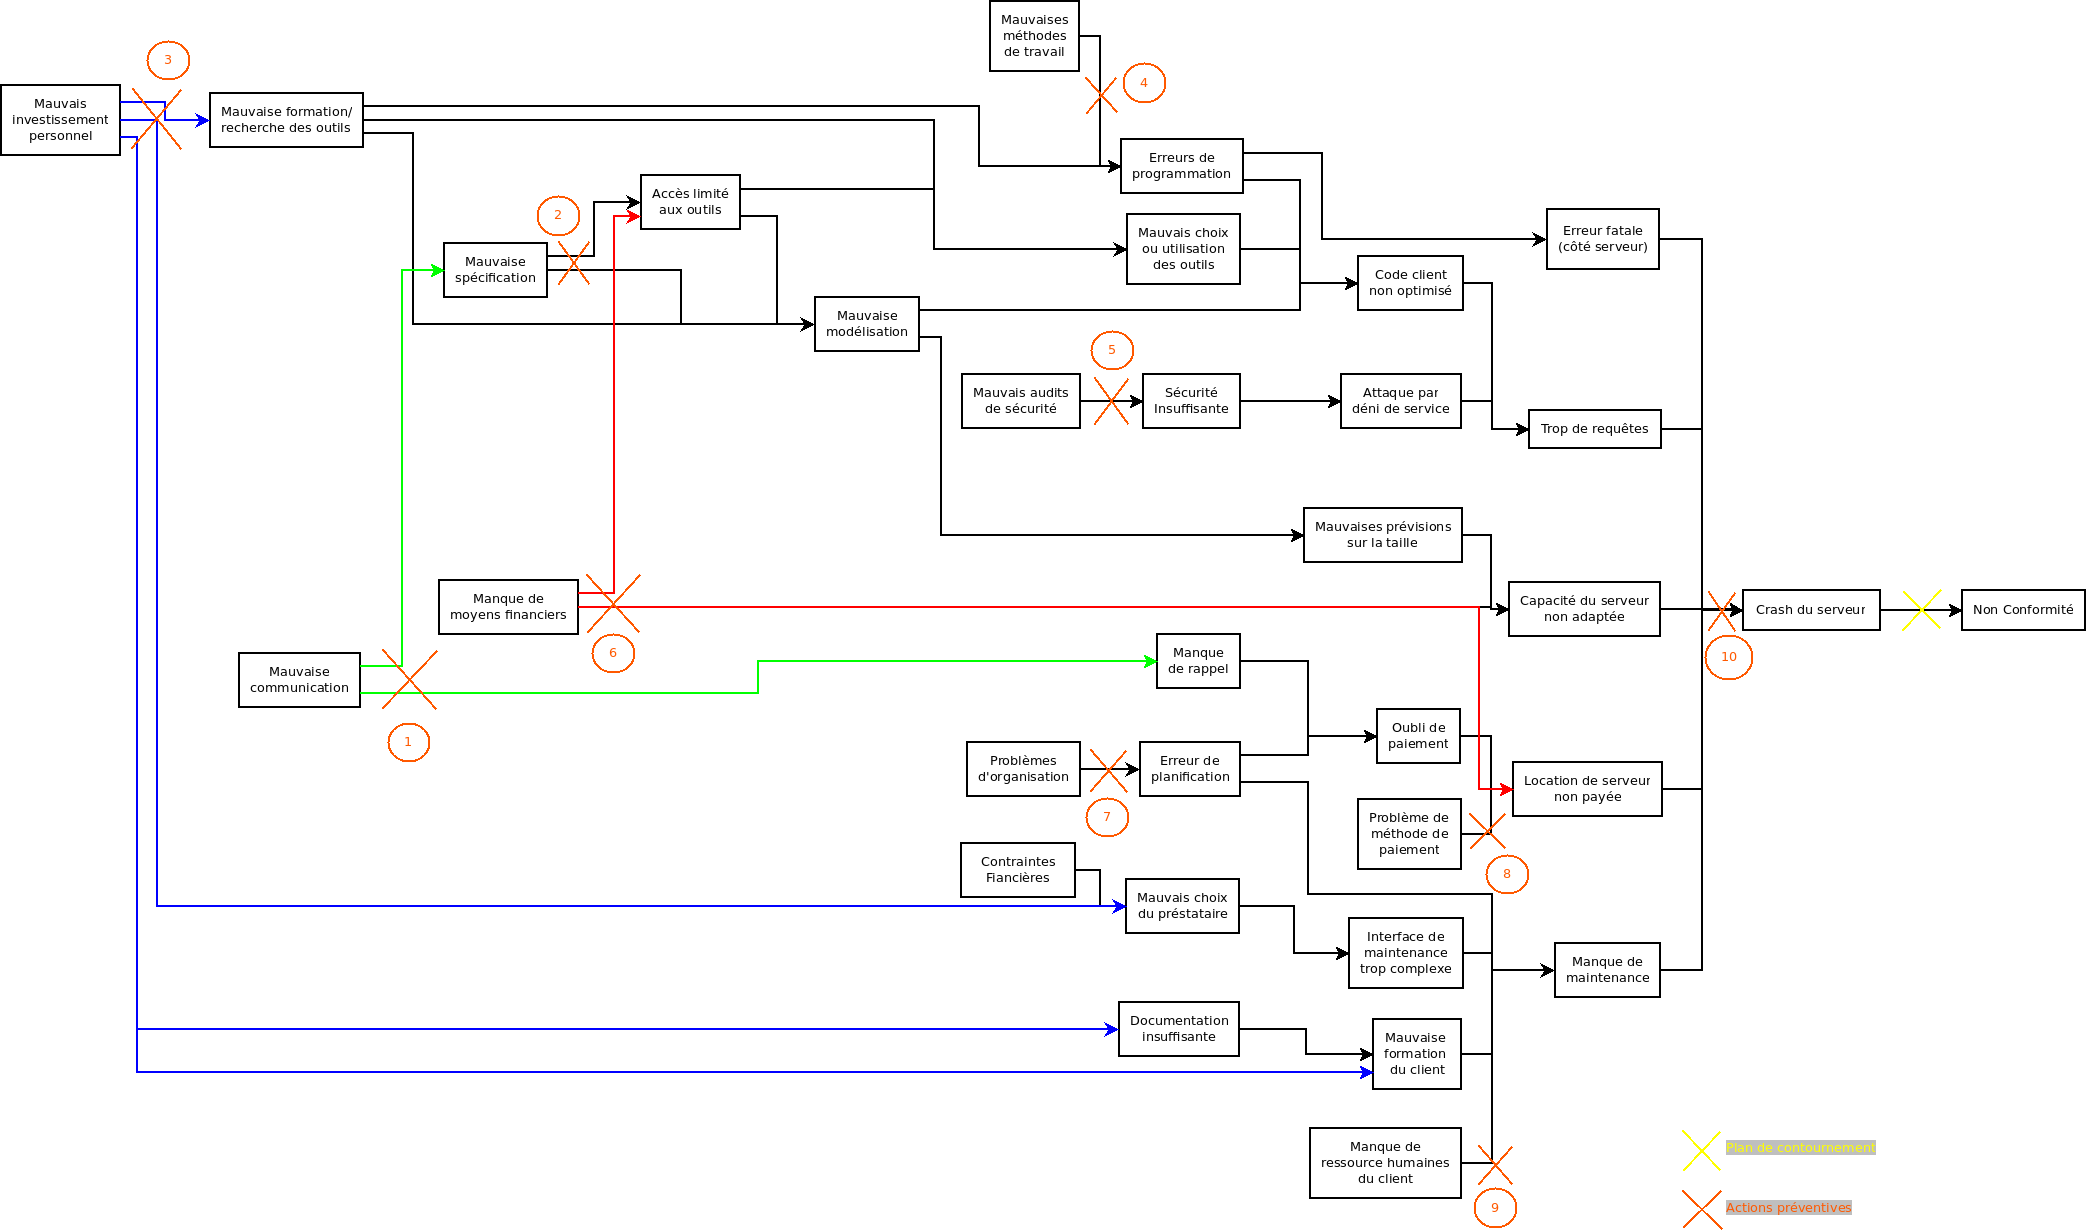
\includegraphics[scale=0.5]{images/AnalyseRisque_nPourquoi_FDR001}
\end{figure}